%set the master document for easy compilation
%!TEX root = ../D3_5_2.tex

%-----------------------------------------------------------------------
\section{Manage ETCS Procedures}
%-----------------------------------------------------------------------
%\tbc
%Baseliyos Jacob

\subsection{Start of Mission - Awakness of Train}%Mainfunction receive track data. Name should be be defined and substituded by the designer of the function. 
\paragraph{Reference to the SRS or other Requirements (or other requirements)}
Chapter 5, § 5.4
\subsubsection{Short descriptoiin of the functionality}
This functionality describes the Start of Mission procedure of the train until the status of the awakness. From this point of the awakness the train will be able to start different modes, levels and further procedure.
See scope of the Start of Mission - Awakness of train in the figure below.

\begin{figure}
\centering
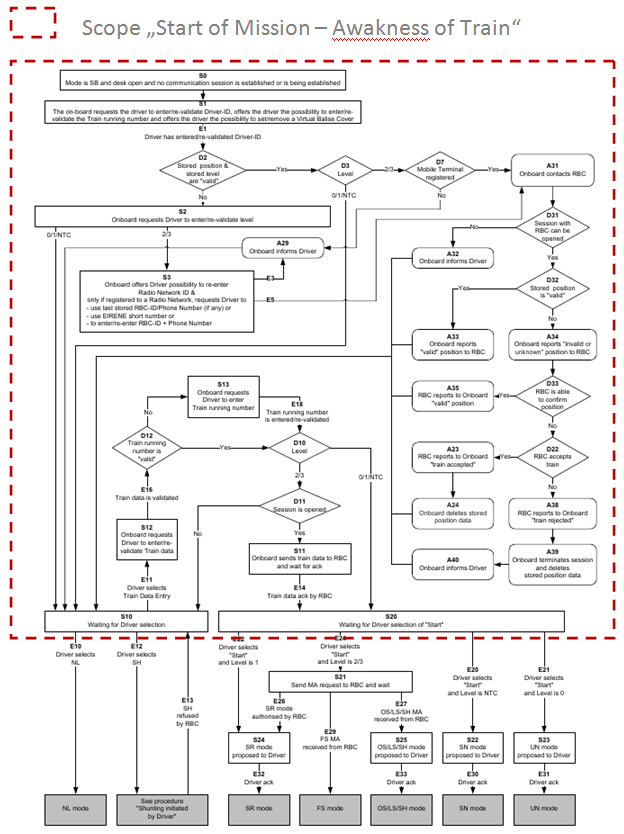
\includegraphics[scale=0.8]{images/SoMAwaknessoftrain}
\caption{Start of Mission - Awakness of Train}
\label{Start of Mission - Awakness of Train}
\end{figure}

\subsubsection{Interface}
\paragraph{Input Flow}
\begin{itemize}
\item Information from TIU
\item Action from Driver (DMI)
\item Information from Position Calculation
\item Information from Persistent Data
\item Information from Management of Radio Communication
\item Information from Mode and Level Management (Level and Mode Status)
\item Information from Radio Block Control
\end{itemize}

\paragraph{Output Flow}
\begin{itemize}
\item Information to Management of Radio Communication
\item Request to Management of Radio Communication
\item Request to Driver (DMI)
\item Request to Mode and Level Management (Request Mode Change)
\item Request to Radio Block Control (Validation of Train Data)
\end{itemize}

\subsubsection{Functional Design Description}
For the third iteration just a part of the Scope has been design. To complete the scenario in the third iteration the ideal path to the awakness of train until the state "waiting for Driver selection of "Start"" have been realized. Furthermore the initial data from the persistend database such as Level, Driver ID, Train Number, Train Data, Radio Number, RBC ID hase been consider as constants. 

\subsubsection{Refernce to the Scade Model}
\url{https://github.com/openETCS/modeling/blob/master/model/Scade/System/ObuFunctions/Procedures/ManageProcedure_Pkg.xscade}

\subsection{Start of Mission in Level 2 or 3 Mode SR FS OS LS SH}

\subsubsection{Reference to the SRS or other Requirements (or other requirements)}
Chapter 5, § 5.4

\subsubsection{Short description of the functionality}
This functionality describes the Start of Mission procedure of the train in Level 2 or 3 and the Modes SR FS OS LS SH where the train under the defined Mode Level supervision starts running.
See scope of the Start of Mission - Level 2 or 3 and Modes SR FS OS LS SH in the figure below.

\begin{figure}
\centering
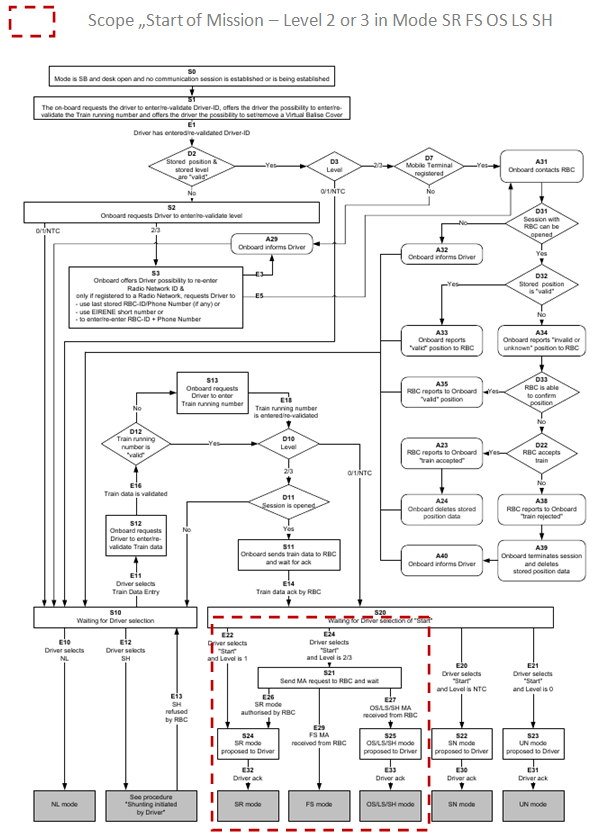
\includegraphics[scale=0.7]{images/SoMLevel2_3_SR_FS_OS_LS_SH}
\caption{Start of Mission - Start of Mission in Level 2 or 3 and Mode SR FS OS LS SH}
\label{Start of Mission - Start of Mission in Level 2 or 3 and Mode SR FS OS LS SH}
\end{figure}


\subsubsection{Interface}
\paragraph{Input Flow}
\begin{itemize}
\item Action from Driver (DMI)
\item Information from Mode and Level Management (Level and Mode Status)
\item Information from Movement Authority Managmement (Receiving of Movement Authority)
\end{itemize}

\paragraph{Output Flow}
\begin{itemize}
\item Request to Driver (DMI)
\item Request to Movement Authority Management (Request Movement Authority)
\item Request to Mode and Level Management (Request Mode Change)
\end{itemize}


\subsubsection{Functional Design Description}
For the third iteration just a part of the Scope has been design. To complete the scenario in the third iteration the path "Full Supervision Movement Authority received from RBC" has been realized. The state will end after the train receives the Change Authority to FS and will be ready to run.

\subsubsection{Refernce to the Scade Model}
\url{https://github.com/openETCS/modeling/blob/master/model/Scade/System/ObuFunctions/Procedures/SoM_SR_FS_OS_LS_SH_SN_UN.xscade}

